

% ****** Start of file aipsamp.tex ****m*
%
%   This file is part of the AIP files in the AIP distribution for REVTeX 4.
%   Version 4.1 of REVTeX, October 2009
%
%   Copyright (c) 2009 American Institute of Physics.
%
%   See the AIP README file for restrictions and more information.
%
% TeX'ing this file requires that you have AMS-LaTeX 2.0 installed
% as well as the rest of the prerequisites for REVTeX 4.1
% 
% It also requires running BibTeX. The commands are as follows:
%
%  1)  latex  aipsamp
%  2)  bibtex aipsamp
%  3)  latex  aipsamp
%  4)  latex  aipsamp
%
% Use this file as a source of example code for your aip document.
% Use the file aiptemplate.tex as a template for your document.
\documentclass[%
 aps, pra,
% jmp,
% bmf,
% sd,
% rsi,
 amsmath,amssymb,
%preprint,%
 reprint,%
%author-year,%
%author-numerical,%
% Conference Proceedings
superscriptaddress
]{revtex4-2}

\usepackage{graphicx}% Include figure files
%\usepackage{dcolumn}% Align table columns on decimal point
\usepackage{bm}% bold math
\usepackage{fixme}
%\usepackage[mathlines]{lineno}% Enable numbering of text and display math
%\linenumbers\relax % Commence numbering lines
\usepackage{hyperref}
\usepackage{kbordermatrix}% http://www.hss.caltech.edu/~kcb/TeX/kbordermatrix.sty
\usepackage[utf8]{inputenc}
\usepackage[T1]{fontenc}
\usepackage{mathptmx}
\usepackage{lipsum}
\usepackage{amsmath}
\usepackage{physics}
\usepackage{xparse}
\usepackage{bbm}
\usepackage{xcolor}
\usepackage{url}


%\usepackage{multirow}
%\usepackage{makecell}
\graphicspath{{Pictures/}}

\renewcommand*{\figureautorefname}{Fig.}
\renewcommand*{\equationautorefname}{Eq.}

\newcommand{\mytitile}{Photon transport in a Bose-Hubbard chain of superconducting artificial atoms}

\begin{document}
	\preprint{AIP/123-QED}
	
	\title[\mytitile]{\mytitile\\~}
	\author{G.P. Fedorov}
	\email{gleb.fedorov@phystech.edu}
	
	\affiliation{ 
		Russian Quantum Center, National University of Science and Technology MISIS, 119049 Moscow, Russia
	}%
	\affiliation{ 
		Moscow Institute of Physics and Technology, Dolgoprundiy, Russia
	}
	\author{S. Remizov}
	\affiliation{Dukhov Automatics Research 
		Institute, (VNIIA), Moscow, Russia}

	\author{I.A. Rodionov}
	\affiliation{FMN Laboratory, Bauman Moscow 
		State Technical University, Moscow, Russia}
	\affiliation{Dukhov Automatics Research 
	Institute, (VNIIA), Moscow, Russia}

	\author{O.V. Astafiev}
	\affiliation{Skolkovo Institute of Science 
		and Technology, Moscow, Russian Federation}
	\affiliation{ 
		Moscow Institute of Physics and Technology, 
		Dolgoprundiy, Russia
	}
	\affiliation{Physics Department, Royal 
	Holloway, University of London, Egham, Surrey 
	TW20 0EX, United Kingdom}
\affiliation{National Physical Laboratory, Teddington, TW11 0LW, United Kingdom}

	\author{A.V. Ustinov}
	\affiliation{ 
		Russian Quantum Center, National University of Science and Technology MISIS, 119049 Moscow, Russia
	}
	\affiliation{Physikalisches Institut, Karlsruhe Institute of Technology, 76131 Karlsruhe, Germany}
	
	
	\date{\today}% It is always \today, today,
	%  but any date may be explicitly specified
	
	
	\begin{abstract}
We investigate non-equilibrium steady-state photon transport through a chain of five coupled artificial atoms described by the Bose-Hubbard model. By increasing incident photon flux, we demonstrate a continuous transition from the linear regime described by the classical coupled oscillators model to the quantum regime of photon blockade characterized by suppressed transmission and complex structure of multiphoton resonances. We show excellent agreement of the transmission with the input-output theory for a model with around a hundred basis states. Next, we demonstrate that our architecture allows straightforward and high-contrast visualization of the emergent energy bands via cross-Kerr spectroscopy. Finally, we show how controllable disorder in the system suppresses this non-local photon transmission. We argue that our architecture may be applied for analog simulation of many-body Floquet dynamics with even larger arrays of artificial atoms paving an alternative way to quantum supremacy.
\end{abstract}
	
\maketitle

\section{Introduction}


There has been increased effort over recent years in analog simulation of various solid state and quantum optical models on a chip using superconducting circuits \cite{kjaergaard2019superconducting}. The Bose-Hubbard (B-H) model is now particularly well-covered as it can be straightforwardly mapped onto arrays of coupled transmons \cite{orell2019probing}. The pioneer work \cite{hacohen2015cooling} had demonstrated this for a three-site linear lattice, and subsequent experiments were focused either on simulating dynamics with engineered dissipation \cite{ma2019dissipatively}, or investigating the many-body localization phase transitions \cite{roushan2017spectroscopic,chiaro2019growth}, or correlated quantum walks \cite{Yan2019, Ye2019}. As numerous theoretical studies propose a new possible research direction involving controllable light-matter interaction and Floquet engineering to study periodically-driven Hamiltonians and their non-equilibrium dynamics \cite{Goldman2014, eisert2015quantum, Zippilli2015, kyriienko2018floquet, franca2020simulating}, it is tempting to use transmon chains  to simulate the driven-dissipative Bose-Hubbard model. The subject is particularly interesting since a recent study has shown that driven systems may open new ways to quantum supremacy \cite{tangpanitanon2019quantum}.

In this Rapid Communication, we present a proof-of-principle device which models non-equilibrium steady-state boson transport through a Bose-Hubbard chain using a linear array of five transmons coupled to waveguides at its edges. We show that continuously driven transmon arrays become very simple to design and control, and thus seem to be suitable for supremacy-scale Floquet quantum simulations. Moreover, the transmission properties of artificial materials composed of qubits attracted theoretical research before \cite{Zagoskin2016, viehmann2013observing, Greenberg2015, Fistul2019, Biella2015} while the corresponding experiments are yet lacking. Finally, we expect that similar simple systems may be useful to test the accuracy of methods of contraction of the Hilbert space such as the matrix product states and tensor networks  \cite{Biella2015, orell2019probing, di2019efficient}.

The layout of the chip is shown in \autoref{fig:scheme}~(a). Similar to previous experiments, we use a chain of directly coupled Xmon transmons tunable via individual flux lines. The distinctive feature is the large interdigitated capacitors to couple the edge transmons strongly to the input and output waveguides and allow measurement of the microwave transmission through the chain. In \autoref{fig:scheme}~(b), we show the physical model that is being simulated by the device. The corresponding Hamiltonian including the classical drive in RWA is
\begin{equation}
\begin{aligned}
\hat H/\hbar &= \sum_{i=1}^5 (\omega_i - \omega_d) \hat b^\dag_i \hat b_i + \frac{1}{2} \alpha_i \hat b_i^\dag \hat b_i (\hat b^\dag_i \hat b_i - 1)\\
&+\sum_{i=1}^4 J (\hat b^\dag_{i+1} \hat b_i + \hat b_{i+1} \hat b_i^\dag)+\frac{\Omega}{2}(\hat b_1^\dag + \hat b_1),
\end{aligned}\label{eq:bose-hubbard}
\end{equation} 
where $\hat b_i$, $\hbar \omega_i$ and $\hbar\alpha_i$ are, respectively, the lowering operator, single-boson energy and the on-site interaction for the $i$\textsuperscript{th} site, $J$ is the inter-site tunneling rate, and $\omega_d$ is the drive frequency. The dissipation in the system is essential to the dynamics as it mostly comes from the waveguides and is included in the corresponding Liouville equation using Lindbladian superoperators $\mathcal D[\hat{O}^{(i)}_\alpha] = \hat{O}^{(i)}_\alpha \hat \rho \hat{O}^{(i)\dag}_\alpha - \frac{1}{2}\{\hat{O}^{(i)\dag}_\alpha \hat{O}^{(i)}_\alpha, \hat \rho\},$ where $\hat{O}^{(i)}_\gamma = \sqrt{\gamma_i} \hat b_i$ is the relaxation and $\hat{O}^{(i)}_\phi = \sqrt{\gamma^{(i)}_\phi} \hat b_i^\dag \hat b_i$ is the pure dephasing. $\gamma_1 = \gamma_5 = \Gamma \gg \gamma_i, \gamma_\phi^{(i)}, i=2,3,4$.


\begin{figure}
	\centering
	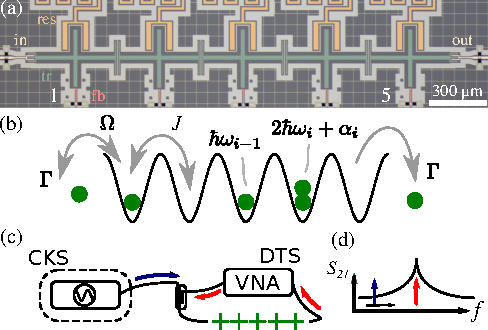
\includegraphics[width=1\linewidth]{Pictures/scheme.pdf}
	\caption{\textbf{(a)} Optical image of the device (false-colored). Input and output waveguides (beige) are strongly coupled to the edge transmons (green), which can be dispersively read out via auxiliary resonators (orange) and tuned via flux lines (red). \textbf{(b)} Interpretation of the device as a B-H lattice with five sites. Bosons are inserted from the left by a drive of strength $\Omega$, and can leak from both sides at rate $\Gamma$. The energy of a localized boson is $\hbar \omega$, and adding another boson to the same site costs $U = \hbar \alpha$. Excitations can tunnel back and forth between sites at rate $J$. \textbf{(c)} Qualitative measurement scheme: the direct transmission (DT) spectroscopy is done using the vector network analyzer which measures the complex transmission $ S_{21} $. The cross-Kerr (C-K) spectroscopy requires an additional microwave source. \textbf{(d)} The C-K spectroscopy is done by sweeping the source frequency (blue arrow) while monitoring the transmission amplitude at some resonance peak via the VNA (red arrow).}
	\label{fig:scheme}
\end{figure}
	

In \autoref{fig:scheme}~(c) we show schematically the experimental setup. We measure the transmission $S_{21}$ through the chain via a vector network analyzer (direct spectroscopy, DT), and optionally use an additional microwave source to perform the cross-Kerr (CK) spectroscopy of the system. Since the microwave signals in our setup are continuous, we are only studying the steady-state properties of the device. To obtain theoretical predictions for the $S_{21}$ in the steady state, one can use the input-output formalism \cite{yurke1984quantum,gardiner1985input}. Since we irradiate the system coherently, we assume that the input field mode amplitude is related to the classical drive strength $\Omega$ in the driving operator $\hbar \Omega \hat b_1 \cos \omega t$ via $\sqrt{\gamma_1} \langle  \hat b_{in}^\dag \rangle \approx i \Omega/2$, which follows from the quantum Langevin equations when disregarding the noise term. Similarly, the output field operator $\hat b_{out}^\dag \approx \sqrt{\gamma_5} \hat b_5^\dag$. From this, we obtain $
	S_{21} = \langle \hat b_{out}^\dag\rangle / \langle \hat b_{in}^\dag \rangle = 2\Gamma\cdot \Tr[\hat \rho_{ss} \hat b_5^\dag]/{i\Omega} ,
$,
where $\hat \rho_{ss}$ is the steadystate density matrix. Physically, this expression means that the signal transmission would be possible if the rightmost transmon becomes excited while the leftmost one is subject to radiation. This apparently non-local excitation of the transmon at the opposite edge of the chain is not a purely quantum-mechanical effect. From the Langevin equations follows that in the limit of zero anharmonicity $\alpha_i = 0$ or, alternatively, $\Omega \ll \Gamma$, the system can be regarded as a chain of classical coupled harmonic oscillators. At the \textit{degeneracy point} when $\omega_i = \omega$, the equivalent classical model still produces transmission peaks at detunings $0,\, \pm J,\, \pm \sqrt{3} J$ from $\omega$, corresponding to the classical normal mode frequencies (see Appendix \ref{sec:app_linear}). In the quantum-mechanical limit, these resonances should remain in the spectrum due to the correspondence principle; however, new lines caused by purely quantum-mechanical processes are expected to appear.

\begin{figure}[b]
	\centering
	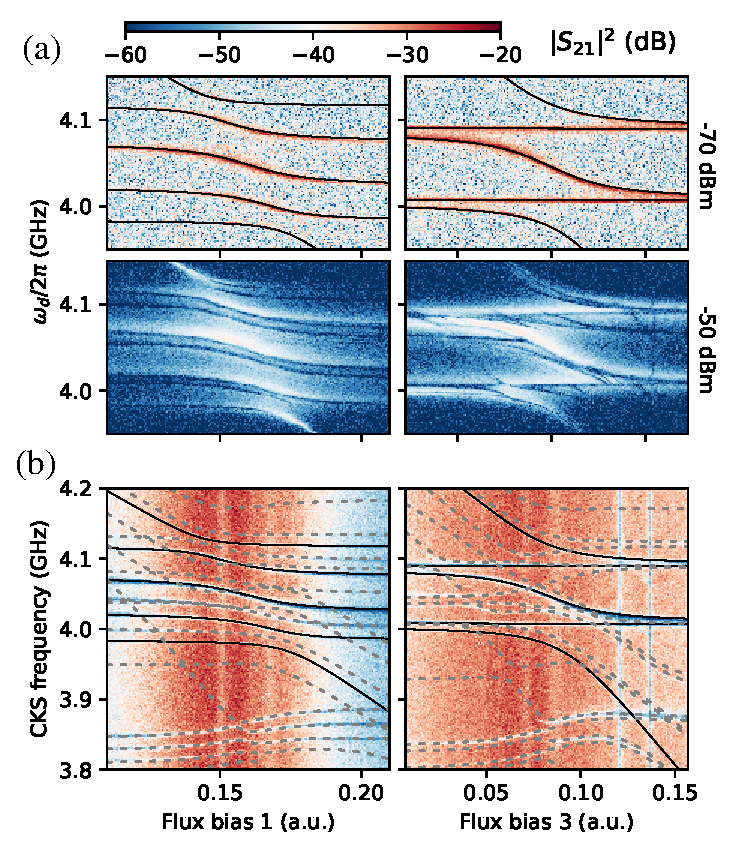
\includegraphics[width=1\linewidth]{Pictures/fig2}
	
	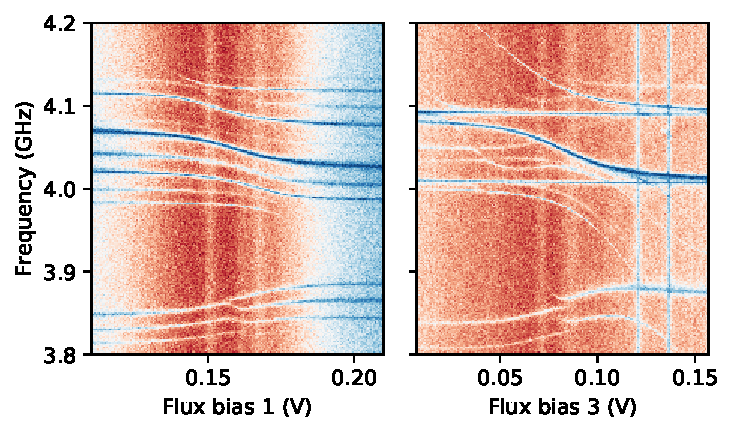
\includegraphics[width=1\linewidth]{Pictures/cktt}
	\caption{\textbf{(a)} Transmission through the chain is observed in five sharp peaks which are shown in dependence on the flux bias voltages 1 (left) and 3 (right) swept around the degeneracy point. In the top row, we show the fit (black lines) of the lowest five transitions of \autoref{eq:bose-hubbard} for $J/2\pi = 41$ MHz, $\omega_i/2\pi \approx 4.05$ GHz ($\Omega = 0$), coinciding with the classical normal modes solution. From top to bottom, as the microwave power is increased (see output power of the VNA on the right), we observe how the system transitions from the classical linear regime to the quantum regime of photon blockade. \textbf{(b)} Cross-Kerr spectroscopy via the the third mode showing the emergent band structure of the system. Dashed lines are fits of the purely quantum transitions with \autoref{eq:bose-hubbard}.}
	\label{fig:transmission}
\end{figure}



\begin{figure*}
	\centering
	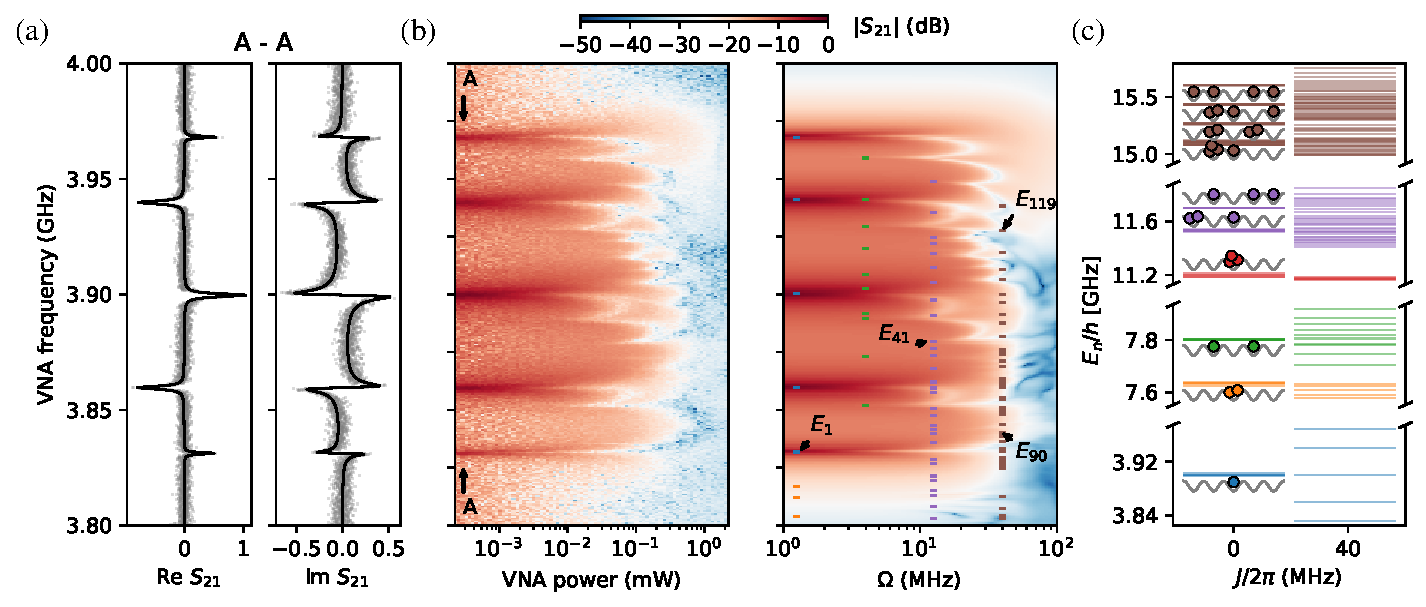
\includegraphics[width=\linewidth]{Pictures/fig3}
	
	
	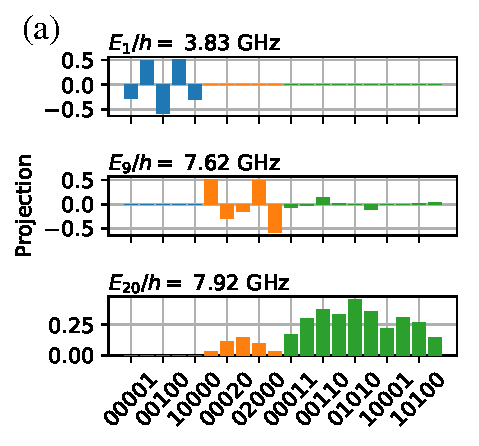
\includegraphics[width=.33\linewidth]{Pictures/eigenstates1}
	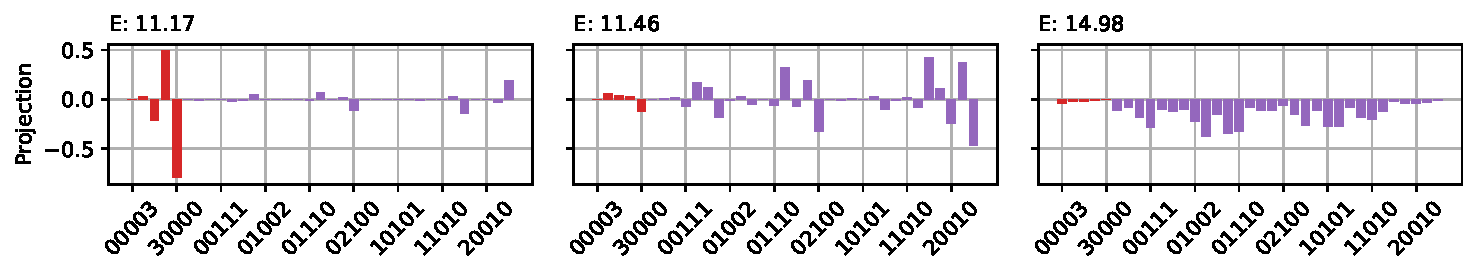
\includegraphics[width=.33\linewidth]{Pictures/eigenstates2}
	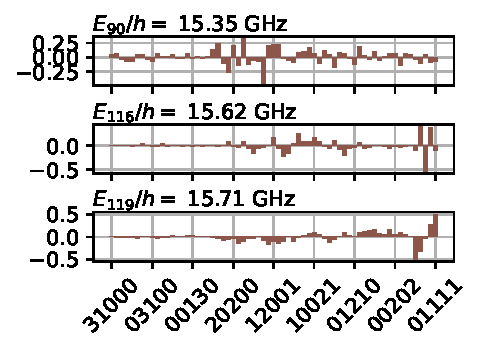
\includegraphics[width=.33\linewidth]{Pictures/eigenstates3}
	\caption{\textbf{(a)} The analytical solution for the $S_{21}$ in the linear regime (smooth curves) fitted to the low power data (clouds), normalized. \textbf{(b)} Experimental and simulated $S_{21}$. The driving power is calibrated to match the corresponding Rabi frequency of the simulation. The observed structure of the multiphoton peaks is reproduced accurately by the numerical model. \textbf{(c)} The energy level structure of the model with and without interaction (model parameters extracted from fits to the data). We take up to three excitations per site, and up to four excitations total. As shown in panel (b) with dashes, these levels are observable in the experiment and are participating in up to four-photon processes. \textbf{(d)} Some reachable eigenstates of the system projected onto the unperturbed basis. An obvious increase of randomness can be seen as the energy grows. }
	\label{fig:cq_transition}
\end{figure*}

The results of the DT spectroscopy are shown in \autoref{fig:transmission}~(a). The plotted transmission amplitude is not normalized, so it includes the attenuation and amplification in the measurement chain. To show the structure of the eigenmodes, we sweep the frequency of one of the transmons across the degeneracy point while keeping the others at around 4.05 GHz. In the left column, the first transmon is swept, and in the right one, the middle one: one can see that the first transmon interacts with all normal modes, and the third only with the odd ones. This behaviour is described exactly by both the classical and quantum mechanics. We find the tunnelling rate $J/2\pi$ to be around 41 MHz from the fit. When the incident power is increased, the resonances are subject to photon blockade \cite{birnbaum2005photon} and behave similarly to what is observed for single superconducting qubits \cite{astafiev2010resonance}. In the bottom row of \autoref{fig:transmission}~(a), we notice spectral manifestations of the many-body states of the system which do not have any classical analogy and cannot be observed in a non-composite quantum system. We thus call this power-dependent behaviour shown in \autoref{fig:transmission}~(a) the classical-to-quantum transition. 


Estimating the parameters of \eqref{eq:bose-hubbard} can be done via the cross-Kerr spectroscopy. In \autoref{fig:transmission}~(b) we have done it using the same two configurations of the transmon frequencies as in \autoref{fig:transmission}~(a) and performed another numerical fit (solid and dashed lines). The readout tone was aimed at the third mode, so the observed spectral frequencies should be corrected by adding it frequency for each bias voltage. The dashed lines show the emergent bands of the two-photon subspace: the many-body states with two excitations at different sites are near 4.05 GHz and ``doublons'' \cite{gorlach2018simulation} are located around 3.85 GHz. The Bose-Hubbard eigenstates with doubly-populated sites have lower energy due to the attractive interactions; extracted values of $U/2\pi$ are approximately [-188, -178, -178, -178, -188] MHz. 
%\section{Classical to quantum transition}
%\begin{figure*}[t]
%	\centering
%	\caption{}
%	\label{fig:eigenstates}
%\end{figure*}

To further study the energy structure and the non-equilibrium dynamics of the system while it transitions from the classical to quantum regime, we use a direct transmission experiment with fixed degenerate configuration of the transmons, $\omega_i/2\pi = 3.9$ GHz. In the linear regime, we estimate the coupling to the transmission lines and internal dissipation from the fit of the complex transmission coefficient predicted by the linear model which is shown in \autoref{fig:cq_transition}~(a). Using these data, we also estimate the overall attenuation in the measurement system and extract only the transmission through the attenuation and amplification chain. We find that the third mode has nearly unity transmission. This is expected, as from \autoref{fig:transmission}~(a) it is only coupled to a single ``bulk'' transmon, and thus has the least internal dissipation. Since in the linear model it is impossible to discern pure dephasing and internal dissipation, the relaxation rates from the fit are larger than true values: we estimate $\gamma_i$ to be [19.9, 1.18, 0.60, 0.95, 18.4] $\mu\text{s}^{-1}$. Also, using the fit we can estimate the disorder in the system; we find $\omega_i/2\pi$ to be [3.878, 3.897, 3.899, 3.902, 3.921] GHz. 

In \autoref{fig:cq_transition}~(b) one can observe the transition from the classical to quantum regime in greater detail: the normal mode peaks gradually saturate due to the photon blockage and the additional dips appear caused by the multiphoton transitions to the many-body eigenstates \cite{Biella2015,PhysRevA.102.013707}. The experimental data agrees very well with the numerical steady-state simulation of the five three-level transmons using the parameters extracted earlier when around 120 relevant eigenstates are included (we put $\gamma_\phi^{(i)} = 0$ since there is no way for us to estimate them independently). The selection rules of the system do not allow all possible multiphoton lines, but we can clearly discern the increase of the density of states and their randomness with increasing band number which is connected to the classical chaotisity of the system if the distribution of the level spacings corresponds to the GOE \cite{bohigas1984characterization,zimmermann1986manifestation, livan2018introduction}. The frequencies of transitions up to four-photon are shown with colored dashes and can be identified with the energy bands shown in \autoref{fig:cq_transition}~(c) calculated using the fitted parameters of the model \eqref{eq:bose-hubbard}. To show how delocalized are the eigenstates reachable in our device, in \autoref{fig:cq_transition}~(d) we project several of them onto the non-interacting basis. State $E_1$ has the structure identical to a classical symmetric low-frequency eigenmode. States $E_{11}$ and $E_{20}$ are at the edges of the orange band of the two-photon subspace and are much larger superpositions. One can note the unveiling randomness in the decomposition coefficients, which becomes more and more pronounced for higher energies: no symmetries or even any kind of structure can be found in the higher eigenstates except for the hole-like four-excitation subspace dual to the single-photon one (see $E_{116, 119}$). We check that the statistics of the calculated nearest-neighbor level spacings resembles the Wigner-Dyson distribution for the experimentally determined parameters, but is Poissonian for the ideal parameters which probably means that the classical motion in that case may be integrable.

\begin{figure}
	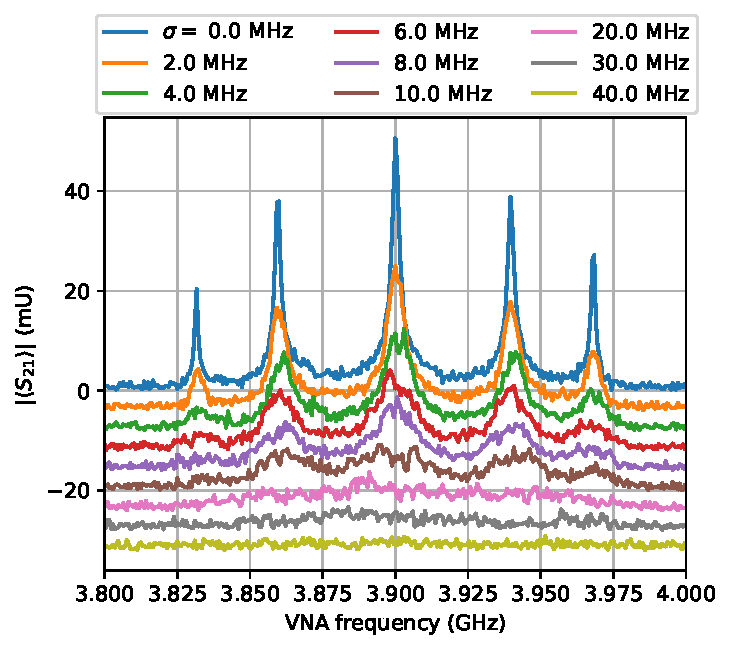
\includegraphics[width=1\linewidth]{Pictures/mbl}
	\caption{\textbf{(a)} Raw transmission data for $\sigma = 6,\, 40$ MHz and 100 realizations of disorder; absolute value of the transmission is shown with color. \textbf{(b)} Localization and disappearance of transmission with increasing disorder. Each curve shows the absolute value of the averaged transmission over the Gaussian disorder realizations with a certain standard deviation $\sigma$ shown in the legend. Each next curve is offset downwards for better visibility.}
	\label{fig:mbl}
\end{figure}

Conversely, it is known that the Poissoinian statistics is usually a property of the disordered Bose-Hubbard model exhibiting localization \cite{roushan2017spectroscopic, Yan2019,Ye2019}. To check how the localization changes the transport properties, we introduce a controllable disorder into the transmon frequencies near the degeneracy point in an experiment similar to what was done before numerically \cite{orell2019probing}: a certain common frequency variance $\sigma$ is chosen, then the random frequency $\omega + \delta \omega$ is assigned to each transmon where $\delta\omega \in \mathbb N(0,2\pi\sigma)$ and $\omega/2\pi = 3.9$ GHz. Then the transmission is recorded, and the full process is repeated 100 times. 
In \autoref{fig:mbl}~(a) we show two examples of the raw transmission data for  $\sigma = 6,\ 40$ MHz. As one can see, for the smaller standard deviation of the target frequencies, the eigenmodes stay relatively unchanged while for the larger the structure is lost completely.

The resulting curves for several values of $\sigma$ are shown in \autoref{fig:mbl}~(b). One can see that when the noise in the transmon frequencies reaches the coupling strength $J/2\pi$, the averaged transmission vanishes. This means that the localization is revealed in the transport properties when the excitation of the first qubit on average does not reach the last qubit. This fact reminds of the superconductor-insulator transition \cite{bruder1993superconductor} for which the Bose-Hubbard model was designed. However, as we only study the lowest excited modes of the system in the linear (classical) regime, one can argue that the observed effect may be equally well described by the classical mechanics. Similarly, even though a system of coupled linear oscillators would not thermalize when a single normal \textit{mode} is excited \cite{deutsch2018eigenstate}, when a single \textit{oscillator} is, the behavior of such system should be identical to the one tested for chains of coupled transmons before \cite{Yan2019, ma2019dissipatively} for low disorder configurations and single-photon states; the observed values would then be not the populations of the single-transmon Fock-states but the amplitudes of the oscillations at each site.

In conclusion, we have shown how classical and quantum photon transport occurs through a Bose-Hubbard chain modelled by a chain of five transmons. We have demonstrated that the behavior of the single-photon subspace of the system does not deviate from the classical normal mode theory which is expected from the correspondence principle. However, an increase of the incident photon flux beyond the dissipation rate reveals the quantum nature of the system through the photon blockade and multiphoton transitions to composite many-body states. The classical theory then fails, and one can only resort to numerical solution of the master equation to find the non-equilibrium steady state, which shows excellent agreement with the data. We have shown how controllable disorder affects the photon transport: we find that the transmission averaged over disorder realizations ceases when the standard deviation of the transmon frequencies reaches the interaction strength. However we want to emphasize that this effect may be explained by the classical mechanics of coupled linear oscillators and quantum many-body localization phenomenon. So a clear distinction should always be made between cases where quantum mechanics is necessary and the classical mechanics is enough.

We gratefully acknowledge valuable discussions with I.S. Besedin and A.V. Ustinov. We thank  A. A. Dobronosova, D. O. Moskalev, A. A. Pishchimova, E. I. Malevannaya for the fabrication of the samples for the experiment. The investigation was conducted with the support of Russian Science Foundation, Grant No. 16-12-00070. Devices/Samples were fabricated at the BMSTU Nanofabrication Facility (Functional Micro/Nanosystems, FMNS REC, ID 74300)


\bibliography{papers_bibliography}% Produces the bibliography via BibTeX.	
\end{document}